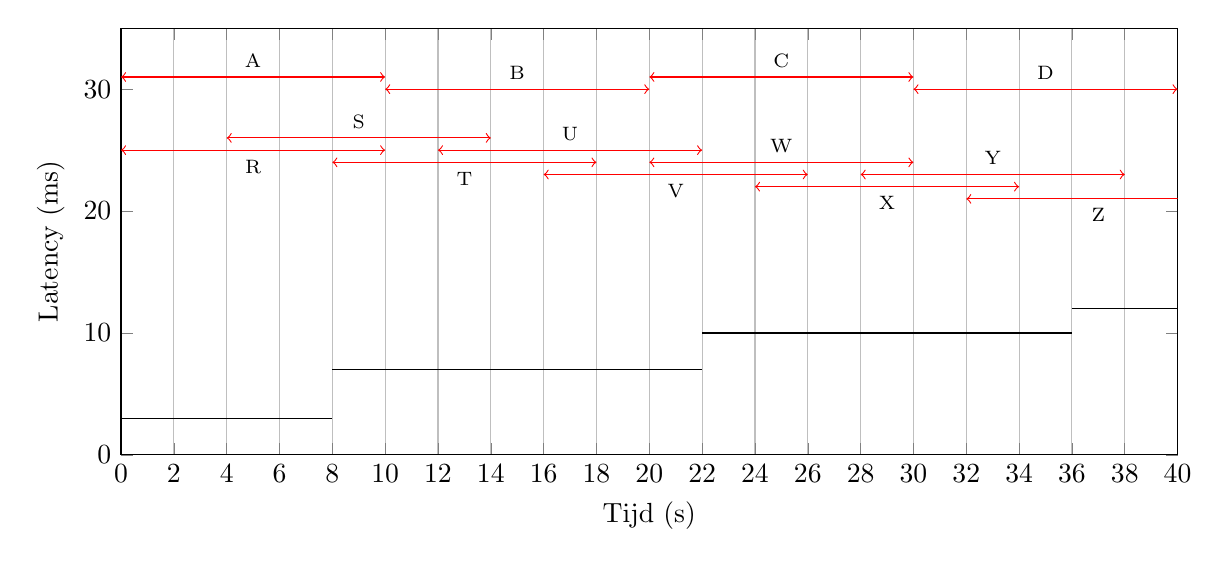
\begin{tikzpicture}[scale=1]
\begin{axis}[
xlabel={Tijd (s)},
ylabel={Latency (ms)},
xmin=0,xmax=40,
ymin=0,ymax=35,
legend style={
	cells={anchor=west},
	legend pos=outer north east,
},
xtick ={0,2,4,6,8,10,...,70},
xmajorgrids=true,
width = 15cm,
height = 7cm
]

after end axis/.code={
	\draw (axis cs:0,3) -- (axis cs:8,3);
	\draw (axis cs:8,7) -- (axis cs:22,7);
	\draw (axis cs:22,10) -- (axis cs:36,10);
	\draw (axis cs:36,12) -- (axis cs:40,12);
	
	\draw[red,<->] (axis cs:0,31) -- (axis cs:10,31)	node [pos=0.5,above,font=\scriptsize,color=black] {A};
	\draw[red,<->] (axis cs:10,30) -- (axis cs:20,30)	node [pos=0.5,above,font=\scriptsize,color=black] {B};
	\draw[red,<->] (axis cs:20,31) -- (axis cs:30,31)	node [pos=0.5,above,font=\scriptsize,color=black] {C};
	\draw[red,<->] (axis cs:30,30) -- (axis cs:40,30)	node [pos=0.5,above,font=\scriptsize,color=black] {D};
	
	\draw[red,<->] (axis cs:0,25) -- (axis cs:10,25)	node [pos=0.5,below,font=\scriptsize,color=black] {R};
	\draw[red,<->] (axis cs:4,26) -- (axis cs:14,26)	node [pos=0.5,above,font=\scriptsize,color=black] {S};
	\draw[red,<->] (axis cs:8,24) -- (axis cs:18,24)	node [pos=0.5,below,font=\scriptsize,color=black] {T};
	\draw[red,<->] (axis cs:12,25) -- (axis cs:22,25)	node [pos=0.5,above,font=\scriptsize,color=black] {U};
	\draw[red,<->] (axis cs:16,23) -- (axis cs:26,23)	node [pos=0.5,below,font=\scriptsize,color=black] {V};
	\draw[red,<->] (axis cs:20,24) -- (axis cs:30,24)	node [pos=0.5,above,font=\scriptsize,color=black] {W};
	\draw[red,<->] (axis cs:24,22) -- (axis cs:34,22)	node [pos=0.5,below,font=\scriptsize,color=black] {X};
	\draw[red,<->] (axis cs:28,23) -- (axis cs:38,23)	node [pos=0.5,above,font=\scriptsize,color=black] {Y};
	\draw[red,<->] (axis cs:32,21) -- (axis cs:42,21)	node [pos=0.5,below,font=\scriptsize,color=black] {Z};
}]

\end{axis}

\end{tikzpicture}